\documentclass{article}

\usepackage[utf8]{inputenc}
\usepackage{mdwlist}
\usepackage[inner=3cm,outer=4cm]{geometry}
\usepackage{mathtools}

\usepackage{Sweave}
\begin{document}
\Sconcordance{concordance:GLMsimIntro.tex:GLMsimIntro.Rnw:%
1 7 1 1 0 9 1 1 2 1 0 2 1 4 0 1 2 2 1 1 2 6 0 1 1 5 0 1 1 5 0 1 1 6 0 1 %
2 2 1 1 2 14 0 1 1 14 0 1 2 12 1 1 2 1 0 1 1 6 0 1 1 12 0 1 1 9 0 1 1 5 %
0 1 1 5 0 1 1 9 0 1 1 5 0 1 2 10 0 1 3 3 1 1 2 15 0 1 1 14 0 1 2 1 0 1 %
1 9 0 1 2 1 0 1 1 9 0 1 1 10 0 1 1 14 0 1 1 15 0 1 2 4 1 1 2 1 0 1 1 14 %
0 1 2 12 1}


\title{GLM simulation. PLS206 Fall 2014}
\author{Emilio A. Laca}
\maketitle

\section{Poisson data}
Imagine we have a known Poisson process that generates random numbers with means equal to 1, 5 and 5 for covariate X values equal to 1, 2 and 3. Let's create a data set with 10 random observations for each level of X.

\begin{Schunk}
\begin{Sinput}
> d1 <- data.frame(mu=rep(c(1,6,7),each=10), X=rep(1:3,each=10))
> d1$Y <- rpois(30,lambda = d1$mu)
> plot(d1$X, d1$Y, pch=16)
\end{Sinput}
\end{Schunk}
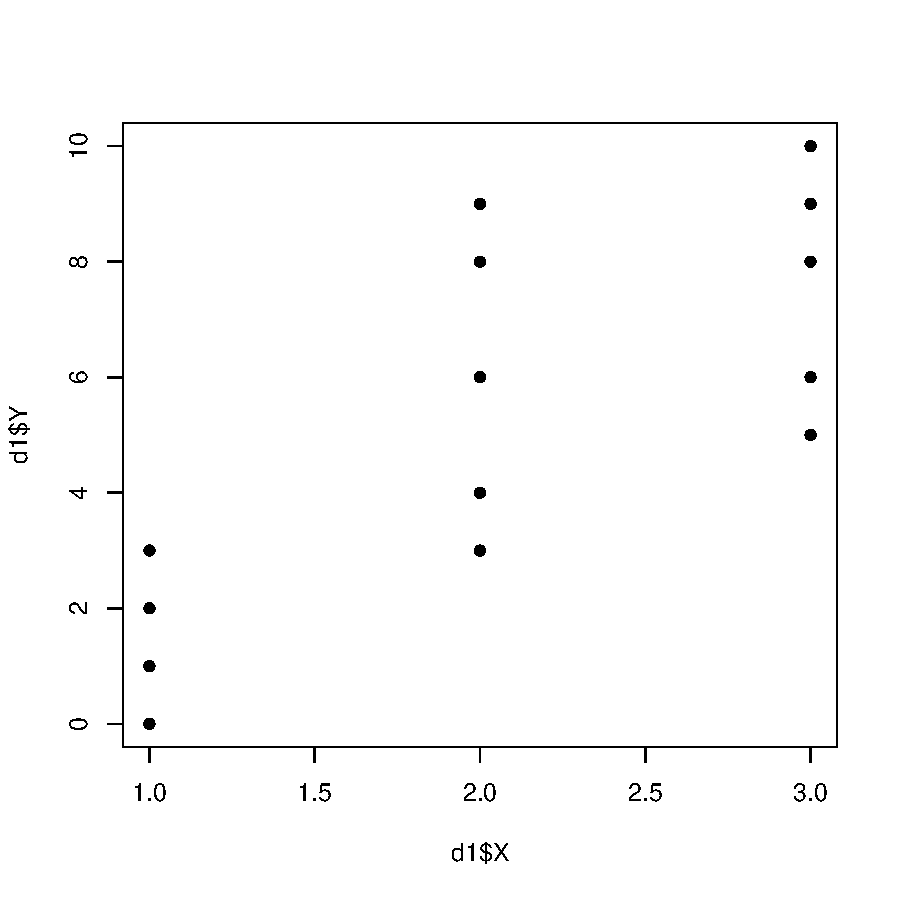
\includegraphics{GLMsimIntro-simData1}

First, let's calculate the deviance for a Saturated model and a minimal or Null model. The saturated model has as many parameters as there are means for the Poisson distribution. We have three different means that we identify with the levels of the covariate X.

\begin{Schunk}
\begin{Sinput}
> print("Residual deviance of the saturated model")
\end{Sinput}
\begin{Soutput}
[1] "Residual deviance of the saturated model"
\end{Soutput}
\begin{Sinput}
> deviance(m.Sat <- glm(Y~factor(X), family="poisson", data=d1))
\end{Sinput}
\begin{Soutput}
[1] 22.67077
\end{Soutput}
\begin{Sinput}
> print("Residual deviance of the Null model")
\end{Sinput}
\begin{Soutput}
[1] "Residual deviance of the Null model"
\end{Soutput}
\begin{Sinput}
> deviance(m.Null <- glm(Y~1, family="poisson", data=d1))
\end{Sinput}
\begin{Soutput}
[1] 69.40559
\end{Soutput}
\end{Schunk}

The saturated model uses three parameters, one $\mu_i$ for each level of X. The set of parameters constitute the vector \textbf{$\beta$} in the linear part of the glm, which has a role practically identical to \textbf{ $\beta$} in linear models in general. We can see how the glm partitions the deviance by looking at the results of the two models:

\begin{Schunk}
\begin{Sinput}
> m.Sat
\end{Sinput}
\begin{Soutput}
Call:  glm(formula = Y ~ factor(X), family = "poisson", data = d1)

Coefficients:
(Intercept)   factor(X)2   factor(X)3  
     0.4055       1.3524       1.6227  

Degrees of Freedom: 29 Total (i.e. Null);  27 Residual
Null Deviance:	    69.41 
Residual Deviance: 22.67 	AIC: 122.6
\end{Soutput}
\begin{Sinput}
> m.Null
\end{Sinput}
\begin{Soutput}
Call:  glm(formula = Y ~ 1, family = "poisson", data = d1)

Coefficients:
(Intercept)  
      1.603  

Degrees of Freedom: 29 Total (i.e. Null);  29 Residual
Null Deviance:	    69.41 
Residual Deviance: 69.41 	AIC: 165.3
\end{Soutput}
\end{Schunk}

For the purpose of developing an intuitive idea of what deviance means, one can think of deviance as residual sum of squares. When the model only has an intercept (overall mean) the deviance is all in the residual. When the model is saturated, all the deviance "explainable" by different parameter values is in the model and the residual is the minimum possible. Deviance is defined as the -2 times the ratio of the likelihood of a model being considered to the likelihood of the saturated model. The deviance scales the likelihood, because the likelihood depends on the number of observations. More observations always lead to smaller probability and likelihood.

\begin{eqnarray}
    deviance = -2 \phi log [(L(model)/L(SaturatedModel)]
    \label{deviance1}
\end{eqnarray}



\section{Understanding likelihood and saturated models}
In order to understand how deviance is calculated we need to understand likelihood and calculate the likelihood of a saturated model. Then, we should be able to retrieve the total deviance of a dataset by calculating the difference between the likelihood of the saturated and the null (intercept only) model. The likelihood is simply the product of the values of the probability density function for each observation given a set of parameter values.

\begin{Schunk}
\begin{Sinput}
> library(likelihood)
> exp(coef(m.Null))
\end{Sinput}
\begin{Soutput}
(Intercept) 
   4.966667 
\end{Soutput}
\begin{Sinput}
> fitted(m.Null)
\end{Sinput}
\begin{Soutput}
       1        2        3        4        5        6        7        8 
4.966667 4.966667 4.966667 4.966667 4.966667 4.966667 4.966667 4.966667 
       9       10       11       12       13       14       15       16 
4.966667 4.966667 4.966667 4.966667 4.966667 4.966667 4.966667 4.966667 
      17       18       19       20       21       22       23       24 
4.966667 4.966667 4.966667 4.966667 4.966667 4.966667 4.966667 4.966667 
      25       26       27       28       29       30 
4.966667 4.966667 4.966667 4.966667 4.966667 4.966667 
\end{Soutput}
\begin{Sinput}
> dpois(d1$Y,exp(coef(m.Null))) # probabilities under minimal null model
\end{Sinput}
\begin{Soutput}
 [1] 0.08592195 0.14224856 0.14224856 0.08592195 0.03459944 0.03459944
 [7] 0.00696633 0.00696633 0.08592195 0.03459944 0.03530418 0.17662529
[13] 0.03530418 0.06397402 0.06397402 0.14224856 0.14523178 0.17662529
[19] 0.17662529 0.14224856 0.03530418 0.17544779 0.01753441 0.17544779
[25] 0.06397402 0.03530418 0.06397402 0.06397402 0.14523178 0.06397402
\end{Soutput}
\begin{Sinput}
> log(prod(dpois(d1$Y,exp(coef(m.Null))))) # likelihood of null model
\end{Sinput}
\begin{Soutput}
[1] -81.64388
\end{Soutput}
\begin{Sinput}
> logLik(m.Null)
\end{Sinput}
\begin{Soutput}
'log Lik.' -81.64388 (df=1)
\end{Soutput}
\begin{Sinput}
> dpois(d1$Y, d1$Y) # probabilities in saturated model
\end{Sinput}
\begin{Soutput}
 [1] 0.2706706 0.2240418 0.2240418 0.2706706 0.3678794 0.3678794 1.0000000
 [8] 1.0000000 0.2706706 0.3678794 0.1317556 0.1953668 0.1317556 0.1395865
[15] 0.1395865 0.2240418 0.1606231 0.1953668 0.1953668 0.2240418 0.1317556
[22] 0.1754674 0.1251100 0.1754674 0.1395865 0.1317556 0.1395865 0.1395865
[29] 0.1606231 0.1395865
\end{Soutput}
\begin{Sinput}
> log(prod(dpois(d1$Y, d1$Y))) # likelihood of saturated model
\end{Sinput}
\begin{Soutput}
[1] -46.94108
\end{Soutput}
\begin{Sinput}
> # deviance is defined as D = 2*phi*(likelihood(sat) - likelihood(mod))
> 2* 1* (log(prod(dpois(d1$Y, d1$Y))) - log(prod(dpois(d1$Y,exp(coef(m.Null))))))
\end{Sinput}
\begin{Soutput}
[1] 69.40559
\end{Soutput}
\begin{Sinput}
> # deviance of null model
\end{Sinput}
\end{Schunk}

A saturated model has a different mean for each observation and thus, it has the maximum possible likelihood for the data. This maximum is taken as the "benchmark" or "baseline" for the data and distribution (Poisson) used: no other model can have greater likelihood. On the other extreme, a model with just one parameter for all observations is the worse sensible model possible. The difference between the best and the worst possible is the deviance available to account for by good models. Good models will account for a lot of that available deviance with few parameters. Now that we have a handle on the total deviance, we can turn to the deviance contributed by each observation, called "deviance residuals."

Deviance residuals are defined as the square root of each term in the sum to calculate the total deviance, each with the sign of the difference between each observation and the corresponding estimated mean.
\begin{Schunk}
\begin{Sinput}
> residuals(m.Sat, type="deviance") # all zero, of course
\end{Sinput}
\begin{Soutput}
          1           2           3           4           5           6 
 0.38823741  1.07651432  1.07651432  0.38823741 -0.43482155 -0.43482155 
          7           8           9          10          11          12 
-1.73205081 -1.73205081  0.38823741 -0.43482155  1.22825074 -0.79214364 
         13          14          15          16          17          18 
 1.22825074  0.86332959  0.86332959 -1.28239082  0.08257494 -0.79214364 
         19          20          21          22          23          24 
-0.79214364 -1.28239082  0.49332944 -1.00642767  0.82990175 -1.00642767 
         25          26          27          28          29          30 
 0.14384961  0.49332944  0.14384961  0.14384961 -0.60277248  0.14384961 
\end{Soutput}
\begin{Sinput}
> residuals(m.Null, type="deviance")
\end{Sinput}
\begin{Soutput}
          1           2           3           4           5           6 
-1.51490144 -0.95315976 -0.95315976 -1.51490144 -2.17435864 -2.17435864 
          7           8           9          10          11          12 
-3.15171911 -3.15171911 -1.51490144 -2.17435864  1.62292794 -0.44910670 
         13          14          15          16          17          18 
 1.62292794  1.24916581  1.24916581 -0.95315976  0.44884282 -0.44910670 
         19          20          21          22          23          24 
-0.44910670 -0.95315976  1.62292794  0.01494038  1.98243706  0.01494038 
         25          26          27          28          29          30 
 1.24916581  1.62292794  1.24916581  1.24916581  0.44884282  1.24916581 
\end{Soutput}
\begin{Sinput}
> # call the set of probabilities for the saturated model pSat
> pSat <- dpois(d1$Y, d1$Y)
> log(pSat)
\end{Sinput}
\begin{Soutput}
 [1] -1.306853 -1.495923 -1.495923 -1.306853 -1.000000 -1.000000  0.000000
 [8]  0.000000 -1.306853 -1.000000 -2.026806 -1.632876 -2.026806 -1.969071
[15] -1.969071 -1.495923 -1.828694 -1.632876 -1.632876 -1.495923 -2.026806
[22] -1.740302 -2.078562 -1.740302 -1.969071 -2.026806 -1.969071 -1.969071
[29] -1.828694 -1.969071
\end{Soutput}
\begin{Sinput}
> # call the set of probabilities for the null model pNull
> pNull <- dpois(d1$Y,exp(coef(m.Null)))
> log(pNull)
\end{Sinput}
\begin{Soutput}
 [1] -2.454316 -1.950179 -1.950179 -2.454316 -3.363918 -3.363918 -4.966667
 [8] -4.966667 -2.454316 -3.363918 -3.343754 -1.733725 -3.343754 -2.749278
[15] -2.749278 -1.950179 -1.929424 -1.733725 -1.733725 -1.950179 -3.343754
[22] -1.740414 -4.043590 -1.740414 -2.749278 -3.343754 -2.749278 -2.749278
[29] -1.929424 -2.749278
\end{Soutput}
\begin{Sinput}
> 2*1*log(pSat/pNull) # squared deviance residuals
\end{Sinput}
\begin{Soutput}
 [1] 2.2949263584 0.9085135196 0.9085135196 2.2949263584 4.7278354848
 [6] 4.7278354848 9.9333333333 9.9333333333 2.2949263584 4.7278354848
[11] 2.6338950883 0.2016968280 2.6338950883 1.5604152117 1.5604152117
[16] 0.9085135196 0.2014598727 0.2016968280 0.2016968280 0.9085135196
[21] 2.6338950883 0.0002232148 3.9300567075 0.0002232148 1.5604152117
[26] 2.6338950883 1.5604152117 1.5604152117 0.2014598727 1.5604152117
\end{Soutput}
\begin{Sinput}
> sign(d1$Y-fitted(m.Null))*sqrt(2*1*log(pSat/pNull))
\end{Sinput}
\begin{Soutput}
          1           2           3           4           5           6 
-1.51490144 -0.95315976 -0.95315976 -1.51490144 -2.17435864 -2.17435864 
          7           8           9          10          11          12 
-3.15171911 -3.15171911 -1.51490144 -2.17435864  1.62292794 -0.44910670 
         13          14          15          16          17          18 
 1.62292794  1.24916581  1.24916581 -0.95315976  0.44884282 -0.44910670 
         19          20          21          22          23          24 
-0.44910670 -0.95315976  1.62292794  0.01494038  1.98243706  0.01494038 
         25          26          27          28          29          30 
 1.24916581  1.62292794  1.24916581  1.24916581  0.44884282  1.24916581 
\end{Soutput}
\begin{Sinput}
> residuals(m.Null)
\end{Sinput}
\begin{Soutput}
          1           2           3           4           5           6 
-1.51490144 -0.95315976 -0.95315976 -1.51490144 -2.17435864 -2.17435864 
          7           8           9          10          11          12 
-3.15171911 -3.15171911 -1.51490144 -2.17435864  1.62292794 -0.44910670 
         13          14          15          16          17          18 
 1.62292794  1.24916581  1.24916581 -0.95315976  0.44884282 -0.44910670 
         19          20          21          22          23          24 
-0.44910670 -0.95315976  1.62292794  0.01494038  1.98243706  0.01494038 
         25          26          27          28          29          30 
 1.24916581  1.62292794  1.24916581  1.24916581  0.44884282  1.24916581 
\end{Soutput}
\end{Schunk}

\section{Binomial regression}

As an example of binominal data we use data on disease incidence in almonds. As they mature, almonds may develop a rot known as hull rot. The data we use are modified from Saa (2014) and are measurements of incidence of hull rot as a function of developmental time and nitrogen fertilization. Data have been randomly modified. Original data are not shown.

\begin{Schunk}
\begin{Sinput}
> d2 <- read.csv("~/Google Drive/PLS206F13/Examples/HW07hrdata.txt", header=TRUE)[,-1]
> d2
\end{Sinput}
\begin{Soutput}
  block nitro nspurs nH
1     2   125     24  3
2     2   350     23 12
3     3   125     24  3
4     3   350     21 10
5     4   125     24  3
6     4   350     24 18
7     5   125     24  1
8     5   350     24  8
\end{Soutput}
\end{Schunk}

\begin{description*}
  \item[block] block indentification number; there were four blocks.
  \item[nitro] level of N fertilization in kg/ha.
  \item[nspurs] total number of spurs marked at the beginning of season.
  \item[nH] number of spurs with hull rot at the end of the season.
\end{description*}

Because there is a set number of spurs observed, the total number of spurs infected is bounded between 0 and the total number of spurs observed. If we assume that each spur is an independent observation with a certain probability of developing hull rot, the final number of spurs infected has a binomial distribution. The linear part of the model specifies that the probability can have effects of block and of nitrogen fertilization.



\end{document}
